\begin{frame}{\texttt{Ironhide}: chains endpoints}

  \includegraphics[page=1,scale=0.2]<1>{res/images/ironhidefinalreview}

  \only<2->{

    \texttt{Ironhide} is the component that manages traffic at
    \textbf{ingress/egress} point of the network

    \vfill{}

    Tasked with packet/flow classification
    \begin{itemize}
      \item Classification based on \textbf{transport layer protocol} used
      \item Performed only at the edges of the chain, not during the traversal
    \end{itemize}

    \vfill{}

    Packets entering/leaving the SFC domain are \textbf{(de)encapsulated}
    accordingly

    \begin{textblock*}{1cm}(10.5cm, 2.5cm)
      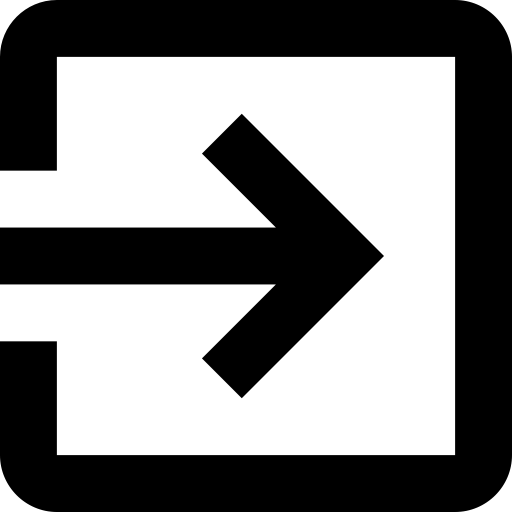
\includegraphics[scale=0.08]{enterexit}
    \end{textblock*}

    \vfill{}

    Keep the connection with the sender/receiver of packets
  }

\end{frame}